
\chapter{Preliminaries}

In this chapter, I introduce fundamental definitions and problems of stringology.
%At the end of the manuscript, I provide a summary of notations.
The reader familiar with basic stringology can skip this chapter and proceed to chapter~\ref{chr:index}.

\section{Definitions}

%I introduce primitive objects of stringology and give basic definitions.

\begin{definition}
\label{def:alpha}
An \emph{alphabet} is a finite ordered set of symbols (or characters).
\end{definition}

\begin{definition}
\label{def:string}
A \emph{string} (or word) over an alphabet is a finite sequence of symbols from that alphabet.
I denote the length of a string $s$ by $|s|$, and by $\epsilon$ the empty string \st $|\epsilon|=0$.
\end{definition}

\begin{definition}
Given an alphabet $\Sigma$, the set $\Sigma^0=\{ \epsilon \}$ contains the empty string, $\Sigma^n$ contains all strings of length $n$ over $\Sigma$, and $\Sigma^* = \cup_{n=0}^{\infty}{\Sigma^n}$ all strings over $\Sigma$.
%Finally, a language over $\Sigma$ is a subset of $\Sigma^*$.
\end{definition}

%\begin{definition}
%The concatenation operator of two strings is defined as $\cdot : \Sigma^* \times \Sigma^* \rightarrow \Sigma^*$.
%Given two strings $x \in \Sigma^m$ with $x=x_1 x_2 \dots x_m$ and $y \in \Sigma^n$ with $y=y_1 y_2 \dots y_n$, their concatenation $x \cdot y$ (or simply $xy$) is the string $z \in \Sigma^{m+n}$ consisting of the symbols $x_1 x_2 \dots x_m y_1 y_2 \dots y_n$.
%\end{definition}
%The notions of prefix, suffix and substring are derived from concatenation.

\begin{definition}
A string $x$ is a \emph{prefix} of another string $y$ iff $x = y_{1 \dots i}$ for some $1 \leq i \leq |y|$.
\end{definition}

\begin{definition}
A string $x$ is a \emph{suffix} of another string $y$ iff $x = y_{i \dots n}$ for some $1 \leq i \leq |y|$.
For convenience, I often denote the suffix of $y$ beginning at position $i$ simply as $y_{i \dots}$.
\end{definition}

\begin{definition} 
A string $x$ is a \emph{substring} of another string $y$ iff $x = y_{i \dots j}$ for some $1 \leq i \leq j \leq |y|$.
\end{definition}

\begin{definition}
A string $x$ \emph{occurs} in another string $y$ iff it is a substring of $y$.
Given $x = y_{i \dots j}$, the occurrence of $x$ starts at position $i$ and ends at position $j$ in $y$.
\end{definition}

%\begin{definition}
%\label{def:subseq}
%A \emph{subsequence} is a non-contiguous sequence of symbols of a given string.
%\end{definition}

\begin{definition}
\label{def:delta}
Given an alphabet $\Sigma$, I define the \emph{distance function} $\delta : \Sigma \times \Sigma \rightarrow \{0, 1\}$ \st $\delta(a,b) = 1$ for any two distinct $a,b \in \Sigma$ and 0 otherwise.
\end{definition}

\begin{definition}
\label{def:rho}
Given an alphabet $\Sigma$ of size $\sigma$, I denote by the function $\rho : \Sigma \rightarrow [1 \dots \sigma]$ the \emph{lexicographic rank} of any alphabet symbol, \st $\rho(a) < \rho(b) \iff a < b$ for any distinct $a,b \in \Sigma$.
\end{definition}

\begin{definition}
\label{def:lex}
The \emph{lexicographical order} $<_{lex}$ between two non-empty strings $x,y$ is defined as $x <_{lex} y \iff x_1 < y_1, \text{ or } x_1 = y_1 \text{ and } x_{2 \dots} <_{lex} y_{2 \dots}$
\end{definition}

%Often in this manuscript I use the notion of string collection.
\begin{definition}
\label{def:colt}
A \emph{string collection} is an ordered multiset $\Sc = \{ s^1, s^2, \dots, s^c \}$ of non necessarily distinct strings over a common alphabet $\Sigma$.
I denote by $\norm{\Sc}=\sum_{i=1}^{c}{|s^i|}$ the total length of the string collection.
I extend the notation of prefix, suffix and substring also to multisets, \eg $\Sc_{(d,i) \dots (d,j)}$ denotes the substring $s^d_{i \dots j}$.
\end{definition}

\begin{definition}
\label{def:dollar}
I call \emph{terminator} a symbol $\$ \not \in \Sigma$ \st $\rho(\$) < \rho(a)$ for any $a \in \Sigma$.
\end{definition}

\begin{definition}
\label{def:strd}
Given a string $s$ over $\Sigma$, I call \emph{padded string} the concatenation of $s$ with a terminator symbol \$.
\end{definition}

\begin{definition}
\label{def:coltd}
Given a string collection $\Sc$ over $\Sigma$, I call \emph{padded string collection} the collection consisting of strings $s^i \in \Sc$ padded with terminator symbols $\$^i$ \st $\rho(\$^i) < \rho(\$^j) \iff i < j$.
\end{definition}

\section{Transcripts, alignments and distances}

I now define the minimal set of edit operations to transform one string into another.
Given two strings $x,y$ of equal length $n$, the string $x$ is easily transformed into the string $y$ by substituting (or replacing) all symbols $x_i$ \st $x_i \neq y_i$ into $y_i$, for $1 \leq i \leq n$.
If the two strings have different lengths, it becomes necessary to insert or delete symbols from $x$ to transform it into $y$.
This fact motivates the following definition of \emph{edit transcript}.

\begin{definition}
\label{def:alignment}
\citep{Gusfield1997} An edit transcript for any two given strings $x,y$ is a finite sequence of substitutions, insertions and deletions transforming $x$ into $y$.
\end{definition}

An \emph{alignment} is an alternative yet equivalent way of visualizing a transformation between strings.
While an edit transcript provides an explicit sequence of edit operations transforming one string into another, an alignment explicitly relates pairs of symbols from the two strings.
Nonetheless, some symbols in one string are not related to any symbol in the other string, \ie when some symbols are inserted or removed.
For this reason, it is necessary to introduce an additional gap symbol $-$ not being part of the string alphabet $\Sigma$.
The definition of alignment follows.
Figure~\ref{fig:edit-transcript} shows an example of edit transcript and alignment.

\begin{definition}
\label{def:alignment}
An alignment of two strings of length $m,n$ over $\Sigma$ is a string of length between $\min\{m,n\}$ and $m+n$ over the pair alphabet $(\Sigma \cup \{ - \}) \times (\Sigma \cup \{ - \})$.
\end{definition}

\begin{figure}[h]
\begin{center}
\caption[Example of edit transcript and alignment]{Example of edit transcript and alignment. The string $x$ is transformed into $y$. The transcript character M indicates a match, R a replacement, I an insertion, and D a deletion.
%The alignment of the strings $x=...$ and $y=...$ is given by the string $z={\text{A} \choose \text{A}}{\text{A} \choose \text{-}}{\text{A} \choose \text{C}}{\text{G} \choose \text{G}}$
}
\label{fig:edit-transcript}
\begin{tikzpicture}[font=\normalsize]

\tikzstyle{n}=[inner sep=0pt, minimum size=10pt, align=center]
\tikzstyle{e}=[-latex, thin]
\tikzstyle{m}=[draw, shape=circle, clabel, pos=0.4, align=center, inner sep=0pt, minimum size=8pt, font=\tiny]
\tikzstyle{t}=[draw, shape=circle, clabel, pos=0.4, align=center, inner sep=0pt, minimum size=8pt, font=\tiny, fill=LightGray]
\tikzstyle{frame}=[draw, rectangle, thin, inner sep=0pt]
\tikzstyle{covered}=[draw, rectangle, thin, inner sep=0pt, fill=LightGray]
\tikzstyle{tape}=[fill=black]
\tikzstyle{strike}=[-, style=double, ultra thin, decorate, decoration=zigzag]
\tikzstyle{line}=[-, thin]
\tikzstyle{wave}=[-, thin, decorate, decoration={snake, segment length=2.5mm, amplitude=0.4mm}]


\newcommand{\transcript}[2]
{
    \foreach[count=\i] \r/\t/\g in {#2}
    {
    	\node[n] (read_\i) at (0.4*\i,0) {\r};
		\node[n] (genome_\i)  at (0.4*\i,-1) {\g};
		\draw[e] (read_\i) -- (genome_\i) node[m] (transcript_\i) {\t};
    }
    
    \begin{pgfonlayer}{background} 
		\draw[tape] ([xshift=0.1cm, yshift=-0.01cm]transcript_1.north west) rectangle ([xshift=-0.1cm, yshift=0.01cm]transcript_#1.south east) ;
	\end{pgfonlayer}
}

\newcommand{\seed}[3]
{
	\ifthenelse{\equal{#3}{0}}
    {
%    	\draw[strike] (read_#1.west) -- (read_#2.east) ;

	    \begin{pgfonlayer}{background} 
    		\draw[covered] (read_#1.north west) rectangle (read_#2.south east) ;
		\end{pgfonlayer}
    }
           
	\node[frame] (read_rect) [transform shape, fit = (read_#1) (read_#2)] {};
}

\newcommand{\band}[1]
{
%	\node[frame] (genome_rect) [transform shape, fit = (genome_1) (genome_#1)] {};

	\draw[line] (genome_1.north west) -- (genome_#1.north east) ;
	\draw[line] (genome_1.south west) -- (genome_#1.south east) ;
	\draw[line] (genome_1.north west) -- (genome_1.south west) ;
	\draw[line] (genome_#1.north east) -- (genome_#1.south east) ;
}

\transcript{25}{G/M/G, C/M/C, T/M/T, N/R/A, T/M/T, G/M/G, G/D/$ $, G/M/G, C/M/C, A/M/A, T/M/T, T/M/T, A/R/G, T/M/T, G/M/G, G/M/G, C/M/C, $ $/I/C, C/M/C, A/M/A, T/M/T, T/M/T, T/M/T, T/R/A, T/M/T}
\band{25}

\node[left=0.25cm of read_1] {$x$} ;
\node[left=0.25cm of genome_1] {$y$} ;
\node[left=0.25cm of transcript_1] {$transcript$} ;

\seed{1}{25}{1}

\end{tikzpicture}
\end{center}
\end{figure}

%A \emph{dotplot} is yet another way to visualize any alignment between two strings and highlight their similarities.
%\begin{definition}
%\label{def:dotplot}
%Given two string $x,y$ of length $m,n$, a dotplot is a $m \times n$ matrix containing a dot at position $(i,j)$ iff the symbol $x_i$ matches symbol $y_j$.
%\end{definition}
%A dotplot trace is a monotonical path in the matrix connecting non-decreasing positions of the matrix.
%Any dotplot trace corresponds to an alignment and vice versa.
%In a trace, match and mismatch columns of the corresponding alignment appear as diagonal stretches, while insertions and deletions are horizontal or vertical stretches.
%See figure~\ref{fig:dotplot}.
%
%\begin{figure}[h]
%\begin{center}
%\caption[Example of dotplot]{Example of dotplot of the strings $x=AAAA$ and $y=CCCC$. The highlighted trace corresponds to the transcript and alignment of figure~\ref{fig:edit-transcript}.}
%\label{fig:dotplot}
%
\begin{tikzpicture}[
	xscale=0.3,yscale=-0.3,
    char/.style={draw=none, text centered, anchor=base},
    position/.style={draw=none, text centered, anchor=base},
]
	\def\CharFont{\small\sffamily}

	\tikzstyle{grid lines}=[gray,densely dotted,line width=0.3pt]
	\tikzstyle{labelstyle}=[font=\sf\footnotesize,color=NumberColor]

	\begin{pgfscope}
		\pgftransformshift{\pgfpoint{-3cm}{0cm}}
		\clip (3,0) rectangle (16, 13);
		\draw[draw=none,fill=gray!2] (1,0) rectangle (16, 13);
		\draw[black] (3,0) rectangle (16, 13);
	\end{pgfscope}

	\PrintDots{0}{0.5}{1,0,1,0,0,0,0,0,0,0,1,0,0}
	\PrintDots{0}{1.5}{0,1,0,0,0,0,0,0,0,0,0,0,1}
	\PrintDots{0}{2.5}{0,1,0,0,0,0,0,0,0,0,0,0,1}
	\PrintDots{0}{3.5}{1,0,1,0,0,0,0,0,0,0,1,0,0}
	\PrintDots{0}{4.5}{0,0,0,1,0,1,0,1,1,0,0,1,0}
	\PrintDots{0}{5.5}{0,0,0,1,0,1,0,1,1,0,0,1,0}
	\PrintDots{0}{6.5}{0,0,0,0,0,0,1,0,0,1,0,0,0}
	\PrintDots{0}{7.5}{0,0,0,1,0,1,0,1,1,0,0,1,0}
	\PrintDots{0}{8.5}{0,0,0,0,0,0,1,0,0,1,0,0,0}
	\PrintDots{0}{9.5}{1,0,1,0,0,0,0,0,0,0,1,0,0}
	\PrintDots{0}{10.5}{0,0,0,1,0,1,0,1,1,0,0,1,0}
	\PrintDots{0}{11.5}{0,1,0,0,0,0,0,0,0,0,0,0,1}
	
	\PrintStringOnly{0}{-1.1}{C,G,C,A,N,A,T,A,A,T,C,A,G}
	\PrintVStringOnly{-1.2}{.5}{C,G,G,C,A,A,T,A,T,C,A,G}
\end{tikzpicture}

%\end{center}
%\end{figure}

%\section{Distance functions}

%A cost is assigned to any alignment, and to its associated edit transformation, by defining a weight function $\delta : (\Sigma \cup \{ - \}) \times (\Sigma \cup \{ - \}) \rightarrow \R_0^{+}$, where:
%\begin{itemize}
%\item $\delta(\alpha,\beta)$ for all $(\alpha,\beta) \in \Sigma \times \Sigma$ defines the cost of substituting $\alpha$ with $\beta$,
%\item $\delta(\alpha,-)$ for all $\alpha \in \Sigma$ defines the cost of deleting the symbol $\alpha$,
%\item $\delta(-,\beta)$ for all $\beta \in \Sigma$ defines the cost of inserting the symbol $\beta$,
%\end{itemize}
%
%The total cost $C(z)$ of an alignment $z$ between two strings is the sum of the weights of all its alignment symbols:
%\begin{eqnarray}
%C(z) = \sum_{i=0}^{|z|}{\delta(z_i)}
%\end{eqnarray}
%Consequently, any distance function $d : \Sigma^{*} \times \Sigma^{*} \rightarrow \R_0^{+}$ takes the minimum cost over all possible alignments of $x,y$:
%\begin{eqnarray}
%d(x,y) = \min_{z \in \mathbb{A}(x,y)}{C(z)}
%\end{eqnarray}

At this point, I define two fundamental distance functions between strings.

\begin{definition}
\label{def:hamming}
\citep{Hamming1950} The \emph{Hamming distance} $d_H : \Sigma^{n} \times \Sigma^{n} \rightarrow \N_0$ between two strings $x,y \in \Sigma^{n}$ counts the number of substitutions necessary to transform $x$ into $y$.
\end{definition}
%I denote the Hamming distance by the function $d_H : \Sigma^{n} \times \Sigma^{n} \rightarrow \N_0$.
%The function $d_H$ is obtained by defining for all $(\alpha,\beta) \in \Sigma \times \Sigma$, $\delta(\alpha,\beta) = 1$ iff $\alpha \neq \beta$ and 0 otherwise, and $\delta(-,\beta)$ to be $+ \infty$ in order to disallow insertions and deletions.

\begin{definition}
\label{def:edit}
\citep{Levenshtein1966} The \emph{Levenshtein} or \emph{edit distance} $d_E : \Sigma^{*} \times \Sigma^{*} \rightarrow \N_0$ between two strings $x,y \in \Sigma^{*}$ counts the \emph{minimum} number of edit operations necessary to transform $x$ into $y$.
\end{definition}
%I denote the edit distance by the function $d_E : \Sigma^{*} \times \Sigma^{*} \rightarrow \N_0$.
%The function $d_E$ is obtained by defining $\delta(\alpha,\beta)$ as for the Hamming distance, and $\delta(\alpha,-) = \delta(-,\beta) = 1$.

The problem of finding an optimal alignment between two strings is equivalent to the problem of finding their minimum distance \citep{Gusfield1997}.
While the Hamming distance between any two strings of length $n$ is easily computed in time $\Oh(n)$, computing the edit distance involves solving a non-trivial optimization problem.

\section{Edit distance computation}

The edit distance between two strings is efficiently computed via \emph{dynamic programming} (DP).
%Below, I describe the three essential components of the DP approach: the recurrence relation, the DP table, and the traceback.
Let $x,y$ be two strings of length $n \geq m$.
The edit distance $d_E(x_{1 \dots i},y_{1 \dots j})$ between any their prefixes $x_{1 \dots i}$ and $y_{1 \dots j}$ is defined recursively.
%for all $1 \leq i \leq m$ and $1 \leq j \leq n$,
The base conditions of the recurrence relation are:
\begin{eqnarray}
d_E(\epsilon,\epsilon)&=&0\label{eq:dp-ee}\\
d_E(x_{1 \dots i},\epsilon)&=&i \; \text{ for all } 1 \leq i \leq n\label{eq:dp-row}\\
d_E(\epsilon, y_{1 \dots j})&=&j \; \text{ for all } 1 \leq j \leq m\label{eq:dp-col}
\end{eqnarray}
and the recursive case for all $1 < i \leq n$ and $1 < j \leq m$ is as follows:
\begin{eqnarray}
d_E(x_{1\dots i},y_{1 \dots j}) = \min \left\{
\begin{array}{lcl}
d_E(x_{1 \dots i-1},y_{1 \dots j})&+&1\\
d_E(x_{1 \dots i},y_{1 \dots j-1})&+&1\\
d_E(x_{1 \dots i-1},y_{1 \dots j-1})&+&\delta(x_i, y_j)
\end{array}
\right.\label{eq:dp-min}
\end{eqnarray}

\begin{figure*}[b!]
\begin{center}
\begin{minipage}[t]{.9\textwidth}
\begin{algorithm}[H]
\Algorithm{EditDistance}{$x,y$}
\begin{tabular}{ll}
\textbf{Input}  & $x$ : string of length $n$\\
				& $y$ : string of length $m$\\
\textbf{Output} & the edit distance $d_E(x,y)$ between $x$ and $y$\\
\end{tabular}
\begin{algorithmic}[1]
\State {$D[0,0] \gets 0$}
\For {$j \gets 1 \, \To m$}
	\State {$D[j,0] \gets D[j-1,0] + 1$}
\EndFor
\For {$i \gets 1 \, \To n$}
	\State {$D[0,i] \gets D[0,i-1] + 1$}
	\For {$j \gets 1 \, \To m$}
		\State {$D[i,j] \gets \min \, \{ \, D[i-1,j] + 1, D[i,j-1] + 1, D[i-1,j-1] + \delta(t_i, p_j) \, \}$}
	\EndFor
\EndFor
\State \Return D[m,n]
\end{algorithmic}
\label{alg:dp-edit}
\end{algorithm}
\end{minipage}
\end{center}
\end{figure*}

Algorithm \ref{alg:dp-edit} computes the above recurrence relation in time $\Oh(nm)$ using a dynamic programming table $D$ of $(n+1) \times (m+1)$ cells, where cell $D[i,j]$ stores the value of $d_E(x_{1 \dots i},y_{1 \dots j})$.
The sole edit distance without any alignment can be computed in space $\Oh(m)$, as only column $D[:j-1]$ is needed to compute column $D[:j]$.
An optimal alignment can be computed in time $\Oh(m + n)$ via \emph{traceback} on the table $D$:
the traceback starts in the cell $D[m,n]$ and goes backwards (either left, up-left, or up) to the previous cell by deciding which condition of equation~\ref{eq:dp-min} yields the value of $D[m,n]$.

%\begin{figure}[h]
%\begin{center}
%\caption[Example of DP table]{DP table representing the computation of the edit distance $d_E(x_{1..5}, y_{1..4})$.}
%\label{fig:edit-dp}
%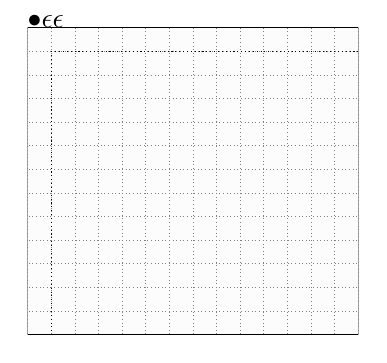
\begin{tikzpicture}[
	xscale=0.3,yscale=-0.3,
    char/.style={draw=none, text centered, anchor=base},
    position/.style={draw=none, text centered, anchor=base}
]

	\begin{pgfscope}
		\pgftransformshift{\pgfpoint{-3cm}{0cm}}
		\clip (3,0) rectangle (17, 13);
		\draw[draw=none,fill=gray!2] (1,0) rectangle (17, 13);
		\draw[style=grid lines](0,0) grid +(20,20);
		\draw[black] (3,0) rectangle (17, 13);
		\draw[black,densely dotted] (4,1) -- (4, 13);
		\draw[black,densely dotted] (4,1) -- (17, 1);
	\end{pgfscope}
	
	\def\CharFont{\scriptsize\sffamily}
	\PrintStringOnly{0}{0.1}{0,1,2,3,4,5,6,7,8,9,10,11,12,13}
	\PrintStringOnly{0}{1.1}{0,1,2,3,4,5,6,7,8,9}
	\PrintStringOnly{0}{2.1}{0,1,2,3,4,5,6,7,8,9}
	\PrintStringOnly{0}{3.1}{0,1,2,3,4,5,6,7,8,9}
	\PrintStringOnly{0}{4.1}{0,1,2,3,4,5,6,7,8,9}
	\PrintStringOnly{0}{5.1}{0,1,2,3,4,5,6,7,8,9}
	\PrintStringOnly{0}{6.1}{0,1,2,3,4,5,6,7,8,$\bullet$}

	\def\CharFont{\small\sffamily}
	\PrintStringOnly{0}{-1.1}{$\epsilon$,C,G,C,A,N,A,T,A,A,T,C,A,G}
	\PrintVStringOnly{-1.2}{0.1}{$\epsilon$,C,G,G,C,A,A,T,A,T,C,A,G}

\end{tikzpicture}

%\end{center}
%\end{figure}


% === Overview of existing methods ===

\section{String matching}

\emph{Exact string matching} is one of the most fundamental problems in stringology.
\begin{definition}
\citep{Gusfield1997}
Given a string $p$ of length $m$, called the \emph{pattern}, and a string $t$ of length $n$, called the \emph{text}, the exact string matching problem is to find all occurrences of $p$ into $t$.
\end{definition}

This problem has been extensively studied from the theoretical standpoint and is well solved in practice \citep{Faro2013}.
Nonetheless, the definition of distance functions between strings lends to a more challenging problem: \emph{approximate string matching}.

\begin{definition}
\citep{Galil1988}
Given a text $t$, a pattern $p$, and a \emph{distance threshold} $k \in \N$, the approximate string matching problem is to find all occurrences of $p$ into $t$ within distance $k$.
\end{definition}
The approximate string matching problem under the Hamming distance is commonly referred as the \emph{$k$-mismatches} problem and under the edit distance as the \emph{$k$-differences} problem.
For $k$-mismatches and $k$-differences, it must hold $k > 0$ as the case $k = 0$ corresponds to exact string matching, and $k < m$ as a pattern trivially occurs at any position in the text if all its $m$ characters are substituted.
Frequently, the problem's input respects the condition $k \ll m \ll n$.
\begin{definition}
Under the edit or Hamming distance, the \emph{error rate} is defined as $\epsilon = \frac{k}{m}$, with $0 < \epsilon < 1$ given the above conditions.
\end{definition}

String matching problems are subdivided in two categories, \emph{online} and \emph{offline}, depending on which string, the pattern or the text, is given first.
Algorithms for online string matching work by preprocessing the pattern and scanning the text from left to right (or right to left).
Algorithms for offline string matching are instead allowed to preprocess the text,
hence they build an index of the text beforehand to speed up subsequent searches.
In practice, if the text is long, static and searched frequently, provided the necessary amount of memory for text indexing, offline methods outperform online methods in terms of runtime.

It goes without saying that offline string matching algorithms are tightly bound to text indexing data structures.
Almost all of these algorithms require a \emph{full-text index}, \ie a data structure representing all substrings of the text.
Very often such \emph{full-text index} is the \emph{suffix tree} \citep{Weiner1973}, a fundamental data structure in stringology.
Among its virtues \citep{Apostolico1985}, the suffix tree natively provides exact string matching in optimal time and approximate string matching via backtracking \citep{Ukkonen1993}.
Often, the suffix tree finds its use within hybrid \emph{filtering methods} rather than on its own.

Filtering methods first discard uninteresting portions of the text and subsequently use a conventional method to verify narrower areas.
These methods work either online or offline.
Online filtering methods try to jump over the text while scanning it; instead, offline filtering methods use an index to place anchors in the text.
Any filtering method relies on a conventional method for verification.
Filtering methods outperform \emph{native} online and indexed methods for a vast range of inputs, \ie when the error rate is low, and are thus very appealing from a practical standpoint.
Nonetheless, filtering methods are just opportunistic combinations of native online and indexed methods.

In this manuscript, I often consider \emph{multiple} string matching problems, \ie variants in which many patterns are given at once, instead of \emph{single} problems where patterns are given one by one in an online fashion.
Obviously, any method for the single case can solve the multiple case and vice versa.
However, it is clear that multiple methods have an advantage over single methods.
For instance, multiple online methods are allowed to preprocess all patterns and then scan the text only once, while single online methods have to scan the text every time a pattern is given.
Thus, provided multiple patterns at once, multiple string matching methods are more appealing than single methods.

In the following of this section, I give a quick overview of the fundamental algorithms and data structures adopted by classic string matching methods.
This overview serves as an introduction to the indexed and filtering methods presented in the next two chapters.
For an extensive treatment of this subject, the reader is referred to complete surveys on online \citep{Navarro2001a} and indexed \citep{Navarro2001} approximate string matching methods.

% --- Online methods ---

\subsection{Online methods}
\label{sub:introonline}

%The most important category of algorithms for approximate string matching are based on dynamic programming.
%DP bit-parallelism.
%Other algorithms for approximate string matching are based on automata \citep{Navarro2001b}.

%\subsubsection{Dynamic programming}

The DP algorithm~\ref{alg:dp-edit} to compute the edit distance between two strings is easily turned into an online $k$-differences algorithm.
Since an occurrence of the pattern can start and end anywhere in the text, approximate string matching consists of computing the edit distance between the pattern and \emph{any substring} of the text.
The problem can be thus solved by computing the distance between the text and the pattern without penalizing leading and trailing deletions in the text.

\begin{figure*}[h]
\begin{center}
\begin{minipage}[t]{.9\textwidth}
\begin{algorithm}[H]
\Algorithm{KDifferences}{$t,p,k$}
\begin{tabular}{ll}
\textbf{Input}  & $t$ : text string of length $n$\\
				& $p$ : pattern string of length $m$\\
				& $k$ : integer bounding the number of errors\\
\textbf{Output} & all end positions of $k$-differences occurrences of $p$ in $t$\\
\end{tabular}
\begin{algorithmic}[1]
\State {$D[0,0] \gets 0$}
\For {$j \gets 1 \, \To m$}
	\State {$D[j,0] \gets j$}
\EndFor
\For {$i \gets 1 \, \To n$}
	\State {$D[0,i] \gets 0$}
	\For {$j \gets 1 \, \To m$}
		\State {$D[i,j] \gets \min \, \{ \, D[i-1,j] + 1, D[i,j-1] + 1, D[i-1,j-1] + \delta(t_i, p_j) \, \}$}
	\EndFor
	\If {$D[i,m] \leq k$}
		\State \Report $i$
	\EndIf
\EndFor
\end{algorithmic}
\label{alg:dp-kdiff}
\end{algorithm}
\end{minipage}
\end{center}
\end{figure*}

Consider the recurrence relation described by equations~\ref{eq:dp-ee}--\ref{eq:dp-min} and pose $x=t$ and $y=p$.
In approximate string matching, an occurrence of the pattern can start anywhere in the text.
Thus, the base condition \ref{eq:dp-row} of the edit distance recurrence relation is changed to:
\begin{eqnarray}
d(x_{1 \dots i}, \epsilon) = 0 \; \text{ for all } 1 \leq i \leq n\label{eq:dp-row-kdiff}
\end{eqnarray}
Thus, algorithm~\ref{alg:dp-kdiff} initializes the top row $D[0:]$ of the DP matrix accordingly
and, since an occurrence of the pattern can end anywhere in the text, it checks any cell in the bottom row for the condition $D[i,m] \leq k$.

%\begin{figure}[h]
%\begin{center}
%\caption[Example of approximate string matching via DP]{DP table representing the match of $p=...$ in $t=...$.}
%\label{fig:asm-dp}
%\begin{tikzpicture}[xscale=0.3,yscale=-0.3]
	\tikzstyle{grid lines}=[gray,densely dotted,line width=0.3pt]
	
	% paralelogram and grid
	\begin{pgfscope}
		\pgftransformshift{\pgfpoint{-3cm}{0cm}}
		\clip (3,0) rectangle (19, 13);
		\draw[draw=none,fill=gray!2] (1,0) rectangle (19, 13);
%		\bandedDotPara{0}{0}{11}{19};
		\fill[fill=DPInitColor] (3,0) rectangle (4,12);
		\fill[fill=DPInitColorDark] (3,12) rectangle (4,13);
		\fill[fill=DPInitColor] (3,0) rectangle (19,1);
		\fill[fill=DPRecurseColor] (4,1) rectangle (19,13);
		\fill[fill=DPRecurseColorDark] (4,12) rectangle (19,13);
		\draw[style=grid lines](0,0) grid +(20,20);
		\draw[black] (3,0) rectangle (19, 13);

		\node at (3.5,0.5) {\sf\tiny \color{DPInitValueColor}0};
		\node at (4.5,0.5) {\sf\tiny \color{DPInitValueColor}0};
		\node at (5.5,0.5) {\sf\tiny \color{DPInitValueColor}0};
		\node at (6.5,0.5) {\sf\tiny \color{DPInitValueColor}0};
		\node at (7.5,0.5) {\sf\tiny \color{DPInitValueColor}0};
		\node at (8.5,0.5) {\sf\tiny \color{DPInitValueColor}0};
		\node at (9.5,0.5) {\sf\tiny \color{DPInitValueColor}0};
		\node at (10.5,0.5){\sf\tiny \color{DPInitValueColor}0};
		\node at (3.5,1.5) {\sf\tiny \color{DPInitValueColor}1};
		\node at (3.5,2.5) {\sf\tiny \color{DPInitValueColor}2};
		\node at (3.5,3.5) {\sf\tiny \color{DPInitValueColor}3};
	\end{pgfscope}
	
	\tikzstyle{labelstyle}=[font=\sf\footnotesize,color=NumberColor]
	
	\node[labelstyle] at (.5,14) {0};
	\node[labelstyle] at (15.5,14) {$n$};
%	\draw[-,color=NumberColor] (-0.45,3.5) -- (-0.15,3.5);

	\node[labelstyle] at (-1,.5) {0};
%	\node[labelstyle,color=black] at (-3,3.5) {$\left\lfloor \frac{m-n+k}{2}\right\rfloor$};
	\node[labelstyle] at (-1,12.5) {$m$};

	\draw[grid lines,fill=DPInitColor]        (17,4)   rectangle +(1,1);
	\draw[grid lines,fill=DPRecurseColor]     (17,5.5) rectangle +(1,1);
%	\draw[grid lines,fill=DPRecurseColorDark] (17,7) rectangle +(1,1);
	\draw[draw=none, fill=DPInitColorDark]    (17,7) -- ++(1,0) -- ++(-1,1) -- ++(0,-1) -- cycle;
	\draw[draw=none, fill=DPRecurseColorDark] (18,7) -- ++(0,1) -- ++(-1,0) -- ++(1,-1) -- cycle;
	\draw[grid lines,fill=none]               (17,7) rectangle +(1,1);
%	\draw[grid lines,fill=gray!2]             (17,8.5)   rectangle +(1,1);
	\node[anchor=base west] at (18,4.85) {\sf\footnotesize initial case};
	\node[anchor=base west] at (18,6.35) {\sf\footnotesize recursive case};
	\node[anchor=base west] at (18,7.85) {\sf\footnotesize tracked score};
%	\node[anchor=base west] at (18,9.35) {\sf\footnotesize ignored};

%	\draw[decorate,decoration={brace,mirror,amplitude=7pt},line width=1pt] (2,5.65) -- (13,5.65) node at (7.5,6.4) [below]{\sf\footnotesize $k+1$} ;

\end{tikzpicture}

%\end{center}
%\end{figure}

% --- Indexed methods ---

\subsection{Indexed methods}
\label{sub:introindex}

%Indexed methods are more attractive than online methods when several patterns are to be searched in the same static text.
%These methods work by building an index of the text beforehand to speed up subsequent searches.
%To this intent,
I now introduce \emph{suffix tries}, idealized data structures to index full-texts.
I define a set of generic operations to traverse them in a top-down fashion.
In chapter~\ref{chr:index}, I expose various data structures replacing suffix tries in practice.
The generic traversal operations here introduced lead to the formulation of generic algorithms that solve string matching problems on any of these data structures.

\subsubsection{Trie}

Consider a padded string collection $\Sc$ (definition~\ref{def:coltd}) consisting of $c$ strings.
Note that padding is necessary to ensure that no string $s^i \in \Sc$ is a prefix of another string $s^j \in \Sc$.
\begin{definition}
The \emph{trie} $\Si$ of $\Sc$ is a lexicographically ordered tree data structure having one node designated as the root and $c$ leaves, denoted as $\Ln_1 \dots \Ln_c$, where leaf $\Ln_i$ points to string $s^i$.
The edge entering any node of $\Si$ is labeled with a symbol in $\Sigma$, while the edge entering any leaf of $\Si$ is labeled with a terminator symbol.
Any path from the root to a leaf $\Ln_i$ spells the string $s^i$, including its terminator symbol $\$^i$.
%Figure~\ref{fig:trie} illustrates.
\end{definition}

\subsubsection{Suffix trie}

\begin{definition}
Given a padded string $s$ (definition~\ref{def:strd}) of length $n$, the suffix trie $\Si$ is the trie of all suffixes of $s$.
The \emph{suffix trie} $\Si$ has $n$ leaves, where leaf $\Ln_i$ points to suffix $s_{i..n}$.
\end{definition}
%The suffix trie generalizes to index string collections.
\begin{definition}
Given a padded string collection $\Sc$ (definition~\ref{def:coltd}), any leaf of the \emph{generalized suffix trie} is labeled with a pair $(i,j)$ where $i$ points to the string $s^i \in \Sc$ and $1 \leq j \leq n_i$ points to one of the $n_i$ suffixes of $s^i$.
Thus each path from the root to a leaf $(i,j)$ spells the suffix $\Sc_{(i,j) \dots}$.
\end{definition}
%Figure~\ref{fig:stree} illustrates.

Note that the (generalized) suffix trie here defined contains $\Oh(n^2)$ nodes, yet I only consider the suffix trie as an idealized data structure to expose generic algorithms.
The optimal data structure to represent in linear space all suffixes of a given string is the \emph{suffix tree} \citep{Morrison1968}.
However, the suffix tree comes with the restriction that internal nodes must have more than one child and with the property that edges can labeled by strings of arbitrary length (see figure~\ref{fig:stree}).
This latter property slightly complicates the exposition of string matching algorithms but it does not affect their runtime complexity nor their result.
For this reason, in the following of this manuscript, I consider \wlogs always suffix tries instead of suffix trees.
%I remark that all given algorithms can be generalized to work on trees.

\begin{figure}[h]
\caption[Example of suffix trie and suffix tree]{Suffix trie and suffix tree of the string {\ttfamily ANANAS\$} .}
\label{fig:stree}
\begin{subfigure}{.5\textwidth}
\begin{center}
\begin{tikzpicture}[scale=1.5,font=\sffamily]

\tikzstyle{level 1}=[sibling distance=12mm, level distance=6mm]
\tikzstyle{level 2}=[sibling distance=6mm, level distance=6mm]
\tikzstyle{level 3}=[sibling distance=6mm, level distance=6mm] 
\tikzstyle{level 4}=[sibling distance=6mm, level distance=6mm] 
\tikzstyle{level 5}=[sibling distance=6mm, level distance=6mm] 
\tikzstyle{level 6}=[sibling distance=6mm, level distance=6mm] 
\tikzstyle{level 7}=[sibling distance=6mm, level distance=6mm] 

%\tikzstyle{transparent}=[edge from parent/.style={draw=none}]
%\tikzstyle{el}=[->,thick,color=gray,text=mycolor1high]

\tikzstyle{transparent}=[edge from parent/.style={draw=none}]
\tikzstyle{el}=[->,thick,color=black,text=black]
\tikzstyle{inner}=[circle,draw,color=black,inner sep=1.5pt]

\node[inner](r) {}
child[transparent] {
node[leaf](D) {$7$}
}
child[transparent] {
node[inner](A) {}
child[transparent] {
node[inner](AN) {}
child[transparent] {
node[inner](ANA) {}
child[transparent] {
node[inner](ANAN) {}
child[transparent] {
node[inner](ANANA) {}
child[transparent] {
node[inner](ANANAS) {}
child[transparent] {
node[leaf](ANANASD) {$1$}
}
}
}
}
child[transparent] {
node[inner](ANAS) {}
child[transparent] {
node[leaf](ANASD) {$3$}
}
}
}
}
child[transparent] {
node[inner](AS) {}
child[transparent] {
node[leaf](ASD) {$5$}
}
}
}
child[transparent] {
node[inner](N) {}
child[transparent] {
node[inner](NA) {}
child[transparent] {
node[inner](NAN) {}
child[transparent] {
node[inner](NANA) {}
child[transparent] {
node[inner](NANAS) {}
child[transparent] {
node[leaf](NANASD) {$2$}
}
}
}
}
child[transparent] {
node[inner](NAS) {}
child[transparent] {
node[leaf](NASD) {$4$}
}
}
}
}
child[transparent] {
node[inner](S) {}
child[transparent] {
node[leaf](SD) {$6$}
}
}
;

\draw[el] (r) -- (D) \labelA{\$};
\draw[el] (r) -- (A) \labelA{A};
\draw[el] (A) -- (AN) \labelA{N};
\draw[el] (AN) -- (ANA) \labelA{A};
\draw[el] (ANA) -- (ANAN) \labelA{N};
\draw[el] (ANAN) -- (ANANA) \labelA{A};
\draw[el] (ANANA) -- (ANANAS) \labelA{S};
\draw[el] (ANANAS) -- (ANANASD) \labelA{\$};
\draw[el] (ANA) -- (ANAS) \labelA{S};
\draw[el] (ANAS) -- (ANASD) \labelA{\$};
\draw[el] (A) -- (AS) \labelA{S};
\draw[el] (AS) -- (ASD) \labelA{\$};

\draw[el] (r) -- (N) \labelA{N};
\draw[el] (N) -- (NA) \labelA{A};
\draw[el] (NA) -- (NAN) \labelA{N};
\draw[el] (NAN) -- (NANA) \labelA{A};
\draw[el] (NANA) -- (NANAS) \labelA{S};
\draw[el] (NANAS) -- (NANASD) \labelA{\$};
\draw[el] (NA) -- (NAS) \labelA{S};
\draw[el] (NAS) -- (NASD) \labelA{\$};
\draw[el] (r) -- (S) \labelA{S};
\draw[el] (S) -- (SD) \labelA{\$};

\end{tikzpicture}

\end{center}
\end{subfigure}%
\begin{subfigure}{.5\textwidth}
\begin{center}
\begin{tikzpicture}[scale=1.5,font=\sf]

\tikzstyle{level 1}=[sibling distance=14mm, level distance=10mm]
\tikzstyle{level 2}=[sibling distance=8mm, level distance=14mm]
\tikzstyle{level 3}=[sibling distance=8mm, level distance=14mm] 

%\tikzstyle{transparent}=[edge from parent/.style={draw=none}]
%\tikzstyle{el}=[->,thick,color=gray,text=mycolor1high]

\tikzstyle{transparent}=[edge from parent/.style={draw=none}]
\tikzstyle{el}=[->,thick,color=black,text=black]
\tikzstyle{inner}=[circle,draw,color=black,inner sep=1.5pt]

\node[inner](r) {}
child[transparent] {
node[inner](A) {}
child[transparent] {
node[inner](ANA) {}
child[transparent] {
node[leaf](ANANAS) {$1$}
}
child[transparent] {
node[leaf](ANAS) {$3$}
}
}
child[transparent] {
node[leaf](AS) {$5$}
}
}
child[transparent] {
node[inner](NA) {}
child[transparent] {
node[leaf](NANAS) {$2$}
}
child[transparent] {
node[leaf](NAS) {$4$}
}
}
child[transparent] {
node[leaf](S) {$6$}
}
;

\draw[el] (r) -- (A) \labelA{A};
\draw[el] (A) -- (ANA) \labelB{N}{A};
\draw[el] (ANA) -- (ANANAS) \labelD{N}{A}{S}{\$};
\draw[el] (ANA) -- (ANAS) \labelB{S}{\$};
\draw[el] (A) -- (AS) \labelB{S}{\$};
\draw[el] (r) -- (NA) \labelB{N}{A};
\draw[el] (NA) -- (NANAS) \labelD{N}{A}{S}{\$};
\draw[el] (NA) -- (NAS) \labelB{S}{\$};
\draw[el] (r) -- (S) \labelB{S}{\$};

\end{tikzpicture}


\end{center}
\end{subfigure}
\end{figure}

\begin{figure}[h]
\caption[Example of generalized suffix trie]{Generalized suffix trie of the string collection $\Sc = \{$ {\ttfamily ANANAS$\$_1$}, {\ttfamily CACAO$\$_2$} $\}$.}
\label{fig:gstrie}
\begin{center}
\begin{tikzpicture}[scale=1.5,font=\sffamily]

\tikzstyle{level 1}=[sibling distance=12mm, level distance=7mm]
\tikzstyle{level 2}=[sibling distance=7mm, level distance=6mm]
\tikzstyle{level 3}=[sibling distance=6mm, level distance=6mm] 
\tikzstyle{level 4}=[sibling distance=6mm, level distance=6mm] 
\tikzstyle{level 5}=[sibling distance=6mm, level distance=6mm] 
\tikzstyle{level 6}=[sibling distance=6mm, level distance=6mm] 
\tikzstyle{level 7}=[sibling distance=6mm, level distance=6mm] 

%\tikzstyle{transparent}=[edge from parent/.style={draw=none}]
%\tikzstyle{el}=[->,thick,color=gray,text=mycolor1high]

\tikzstyle{transparent}=[edge from parent/.style={draw=none}]
\tikzstyle{el}=[->,thick,color=black,text=black]
\tikzstyle{inner}=[circle,draw,color=black,inner sep=1.5pt]

\node[inner](r) {}
child[transparent] {
node[leaf](D) {$1,7$}
}
child[transparent] {
node[leaf](D2) {$2,6$}
}
child[transparent] {
node[inner](A) {}
child[transparent] {
node[inner](AC) {}
child[transparent] {
node[inner](ACA) {}
child[transparent] {
node[inner](ACAO) {}
child[transparent] {
node[leaf](ACAOD) {$2,2$}
}
}
}
}
child[transparent] {
node[inner](AN) {}
child[transparent] {
node[inner](ANA) {}
child[transparent] {
node[inner](ANAN) {}
child[transparent] {
node[inner](ANANA) {}
child[transparent] {
node[inner](ANANAS) {}
child[transparent] {
node[leaf](ANANASD) {$1,1$}
}
}
}
}
child[transparent] {
node[inner](ANAS) {}
child[transparent] {
node[leaf](ANASD) {$1,3$}
}
}
}
}
child[transparent] {
node[inner](AO) {}
child[transparent] {
node[leaf](AOD) {$2,4$}
}
}
child[transparent] {
node[inner](AS) {}
child[transparent] {
node[leaf](ASD) {$1,5$}
}
}
}
child[transparent] {
node[transparent](XXX) {}
}
child[transparent] {
node[inner](C) {}
child[transparent] {
node[inner](CA) {}
child[transparent] {
node[inner](CAC) {}
child[transparent] {
node[inner](CACA) {}
child[transparent] {
node[inner](CACAO) {}
child[transparent] {
node[leaf](CACAOD) {$2,1$}
}
}
}
}
child[transparent] {
node[inner](CAO) {}
child[transparent] {
node[leaf](CAOD) {$2,3$}
}
}
}
}
child[transparent] {
node[inner](N) {}
child[transparent] {
node[inner](NA) {}
child[transparent] {
node[inner](NAN) {}
child[transparent] {
node[inner](NANA) {}
child[transparent] {
node[inner](NANAS) {}
child[transparent] {
node[leaf](NANASD) {$1,2$}
}
}
}
}
child[transparent] {
node[inner](NAS) {}
child[transparent] {
node[leaf](NASD) {$1,4$}
}
}
}
}
child[transparent] {
node[inner](O) {}
child[transparent] {
node[leaf](OD) {$2,5$}
}
}
child[transparent] {
node[inner](S) {}
child[transparent] {
node[leaf](SD) {$1,6$}
}
}
;

\draw[el] (r) -- (D) \labelA{$\$_1$};
\draw[el] (r) -- (D2) \labelA{$\$_2$};

\draw[el] (r) -- (A) \labelA{A};
\draw[el] (A) -- (AC) \labelA{C};
\draw[el] (AC) -- (ACA) \labelA{A};
\draw[el] (ACA) -- (ACAO) \labelA{O};
\draw[el] (ACAO) -- (ACAOD) \labelA{$\$_2$};

\draw[el] (A) -- (AN) \labelA{N};
\draw[el] (AN) -- (ANA) \labelA{A};
\draw[el] (ANA) -- (ANAN) \labelA{N};
\draw[el] (ANAN) -- (ANANA) \labelA{A};
\draw[el] (ANANA) -- (ANANAS) \labelA{S};
\draw[el] (ANANAS) -- (ANANASD) \labelA{$\$_1$};
\draw[el] (ANA) -- (ANAS) \labelA{S};
\draw[el] (ANAS) -- (ANASD) \labelA{$\$_1$};
\draw[el] (A) -- (AO) \labelA{O};
\draw[el] (AO) -- (AOD) \labelA{$\$_2$};
\draw[el] (A) -- (AS) \labelA{S};
\draw[el] (AS) -- (ASD) \labelA{$\$_1$};

\draw[el] (r) -- (C) \labelA{C};
\draw[el] (C) -- (CA) \labelA{A};
\draw[el] (CA) -- (CAC) \labelA{C};
\draw[el] (CAC) -- (CACA) \labelA{A};
\draw[el] (CACA) -- (CACAO) \labelA{O};
\draw[el] (CACAO) -- (CACAOD) \labelA{$\$_2$};
\draw[el] (CA) -- (CAO) \labelA{O};
\draw[el] (CAO) -- (CAOD) \labelA{$\$_2$};

\draw[el] (r) -- (N) \labelA{N};
\draw[el] (N) -- (NA) \labelA{A};
\draw[el] (NA) -- (NAN) \labelA{N};
\draw[el] (NAN) -- (NANA) \labelA{A};
\draw[el] (NANA) -- (NANAS) \labelA{S};
\draw[el] (NANAS) -- (NANASD) \labelA{$\$_1$};
\draw[el] (NA) -- (NAS) \labelA{S};
\draw[el] (NAS) -- (NASD) \labelA{$\$_1$};
\draw[el] (r) -- (O) \labelA{O};
\draw[el] (O) -- (OD) \labelA{$\$_2$};

\draw[el] (r) -- (S) \labelA{S};
\draw[el] (S) -- (SD) \labelA{$\$_1$};

\end{tikzpicture}

\end{center}
\end{figure}

\subsubsection{Top-down traversal}

I define a set of generic operations to traverse tries in a top-down fashion.
Given a trie $\Ti$, I define the following operations inspecting any pointed node $\Tn$ of $\Ti$:
\begin{itemize}
\item \textsc{isRoot}($\Tn$) returns true iff the pointed node is the root;
\item \textsc{isLeaf}($\Tn$) returns true iff all outgoing edges are labeled by terminator symbols;
\item \textsc{label}($\Tn$) returns the symbol labeling the edge entering $\Tn$;
\item \textsc{occurrences}($\Tn$) returns the list of positions pointed by leaves below $\Tn$;
\end{itemize}
and the following operations moving from pointed node $\Tn$, and returning true on success and false otherwise:
\begin{itemize}
\item \textsc{goDown}($\Tn$) moves to the lexicographically smallest child of $\Tn$;
\item \textsc{goDown}($\Tn, c$) moves to the child of $\Tn$ whose entering edge is labeled by $c$;
\item \textsc{goRight}($\Tn$) moves to the lexicographically next child of $\Tn$;
\item \textsc{goUp}($\Tn$) moves to the parent node of $\Tn$.
\end{itemize}

Time complexities of the above operations depend on the data structure implementing the trie.
Usually \textsc{label} is $\Oh(1)$, both variants of \textsc{goDown} and \textsc{goRight} can be $\Oh(1)$ or logarithmic in $n$, \textsc{occurrences} can be linear in the number of occurrences, \textsc{goUp} is $\Oh(1)$ but with an additional $\Oh(n)$ space complexity to stack all parent nodes.
Algorithms \ref{alg:st-godown} and \ref{alg:st-goright} show how to implement respectively \textsc{goDown} and \textsc{goRight} using \textsc{goDown} a symbol and \textsc{goUp}, although with a worst-case time complexity of $\Oh(\sigma)$.
In chapter~\ref{chr:index}, I consider various data structures to implement suffix tries, I show how to implement these operations and give their complexities.

\begin{figure*}
\begin{minipage}[t]{.5\textwidth}
\begin{algorithm}[H]
\Algorithm{goDown}{$\Tn$}
\begin{tabular}{ll}
\textbf{Input}  & $\Tn$ : pointer to a suffix trie node\\
\textbf{Output} & boolean indicating success\\
\end{tabular}
\begin{algorithmic}[1]
\If {\Call{isLeaf}{$\Tn$}}
	\State \Return \False
\EndIf
\If {\Call{goDown}{$\Tn, \min_{lex}{\Sigma}$}}
	\State \Return \True
\Else
	\State \Return $\Call{goRight}{$\Tn$}$		
\EndIf
\end{algorithmic}
\label{alg:st-godown}
\end{algorithm}
\end{minipage}
\hfill
\begin{minipage}[t]{.5\textwidth}
\begin{algorithm}[H]
\Algorithm{goRight}{$\Tn$}
\begin{tabular}{ll}
\textbf{Input}  & $\Tn$ : pointer to a suffix trie node\\
\textbf{Output} & boolean indicating success\\
\end{tabular}
\begin{algorithmic}[1]
\If {\NotB \Call{isRoot}{$\Tn$}}
	\While {$c \gets \text{next}_{lex}{\Sigma,\Call{label}{\Tn}}$}
		\State {$\Call{goUp}{x}$}
		\If {$\Call{goDown}{x, c}$}
			\State \Return \True
		\EndIf
	\EndWhile
\EndIf
\State \Return \False
\end{algorithmic}
\label{alg:st-goright}
\end{algorithm}
\end{minipage}
\end{figure*}


% --- Filtering methods ---

\subsection{Filtering methods}
\label{sec:intro:filtering}

Filtering methods work in two stages: the \emph{filtration stage} discards portions of the text unlikely or unable to contain an occurrence of the pattern, subsequently the \emph{verification stage} checks the remaining portions.
The filtration stage proceeds online by scanning the text or alternatively offline using an index of the text.
The verification stage uses a conventional method, \eg the online dynamic programming method or some variation of it.
The crux of filtering methods is thus to accurately and efficiently classify text portions as containing or not an occurrence of the pattern.

\begin{table}[h]
\begin{center}
\caption[Classification of text locations by filtering methods]{Classification of text locations by filtering methods.}
\begin{tabular}{ccc}
\toprule
Occurrence & Filtered in & Filtered out\\
\midrule
Yes & True positive (TP) & False negative (FN) \\
No & False positive (FP) & True negative (TN) \\
\bottomrule
\end{tabular}
\label{tab:filter:accuracy}
\end{center}
\end{table}

\subsubsection{Specificity and sensitivity}

Any filtering method is thus a binary classification method.
Any text location is \emph{true} if it coincides with the beginning of an occurrence of the pattern and \emph{false} if it does not.
The outcome of the classification method is \emph{positive} for text locations filtered in and \emph{negative} for locations filtered out.
Therefore, as shown in table \ref{tab:filter:accuracy}, any text location represents either a \emph{true positive} (TP), a \emph{false positive} (FP), a \emph{true negative} (TN), or a \emph{false negative} (FN).
Standard \emph{specificity} and \emph{sensitivity} measure the accuracy of filtering methods.
The specificity of a filter is defined as:
\begin{eqnarray}
\frac{|TN(t)|}{|TN(t)| + |FP(t)|}
\end{eqnarray}
and the sensitivity as:
\begin{eqnarray}
\frac{|TP(t)|}{|TP(t)| + |FN(t)|}
\end{eqnarray}

%An important case is its sensitivity is 1.
\begin{definition}
A filter is \emph{lossless} or \emph{full-sensitive} if its sensitivity is 1, \ie it produces no false negatives, otherwise it is \emph{lossy}.
\end{definition}
%A full-sensitive filter for approximate string matching solves the problem exactly.
Many practical applications, \eg read mapping do not require strictly lossless filtration.
Nonetheless, a predictable or controlled lossy filter helps to interpret the results and insure their quality.
For this reason, I focus on criteria yielding filters which are lossless or lossy in a predictable fashion.

\subsubsection{Efficiency}

The total runtime of a filtering method is given by the sum of the runtimes of its filtration and verification stages.
Filtration specificity determines how much time goes in the verification stage.
Clearly, the number of false positives must be low to keep verification time small.
Nonetheless, the filtration stage must also run in a reasonable amount of time.
Hence, an efficient filtering method balances its runtime between filtration and verification.
In any way, no filtering method can be efficient when the number of true positive locations approaches the text length.
%No filtering method is effective unless $|TP(t)| \ll |t|$.

Filtering methods for string matching work under the assumption that patterns occur in the text with a \emph{low average probability}.
For $k$-differences, the occurrence probability is a function of the error rate $\epsilon$, in addition to the alphabet size $\sigma$, and can be computed or estimated under the assumption of the text being generated by a specific random source.
Under the uniform Bernoulli model, where each symbol of $\Sigma$ occurs with probability $\frac{1}{\sigma}$, \citeauthor{Navarro2000} estimate that $\epsilon < 1 - \frac{1}{\sigma}$ is a conservative bound on the error rate which ensures few occurrences and for which filtering algorithms are effective.
For higher error rates, non-filtering methods, either online or offline, work better.

\subsubsection{Seeds versus $q$-grams}

Filtering methods apply combinatorial criteria to determine which portions of the text might contain some occurrence of the pattern.
These criteria are in general valid for both online and offline variants of the problem.
In practice, one specific criterion might be more convenient for one variant of the problem rather than the other.
The combinatorial criterion underlying a filter is of paramount importance as it provides guarantees on filtration sensitivity.

In chapter \ref{sec:filter}, I consider two classes of combinatorial filtering methods: those based on \emph{seeds} and those based on \emph{$q$-grams}.
Filters in the former class partition the pattern into \emph{non-overlapping} factors called seeds.
Application of the pigeonhole principle yields full-sensitive partitioning strategies.
Instead, filters in the latter class consider all \emph{overlapping} substrings of the pattern having length $q$, the so-called $q$-grams.
Simple counting lemmata give lower bounds on the number of $q$-grams that must be present in a narrow window of the text, as necessary condition for an approximate occurrence of the pattern.
